\section{Learned Street-Level Risk, and Routing People Around Water}
\label{sec:gnn}

Both planning surfaces above route on graphs with hand-set costs. We now replace the hand-set cost
with a learned one, and in doing so answer a different question. A planner asks where to build. A
person standing in the rain asks which way to walk.

\subsection{FloodGNN}
FloodGNN is an edge-conditioned message-passing network \cite{gilmer2017} over the OpenStreetMap
street graph, with four rounds of message passing, 96-dimensional states and about 439\,k
parameters. Message passing means each street repeatedly exchanges information with the streets it
connects to, so a street can learn that it is at the bottom of a basin even though nothing in its
own features says so. The network is conditioned on rainfall by FiLM \cite{perez2018film}, which
lets one model cover a continuous range of storm sizes instead of one model per storm.

Node features are deliberately local and standardised per graph. They are elevation anomaly,
pit-ness, grade, flow accumulation, permanent water, radar waterlogging frequency, and building and
road density. Nothing in them identifies the city, which is the property that makes transfer
possible at all.

Supervision is generated by the twin itself. The emulator's depth fields over a 20 to 240\,mm sweep
are sampled at street nodes and edges, and the drain planner's conveyed volume is sampled at three
configurations. That is about nine seconds of label generation per city on a CPU. Wet targets carry
the same twenty-fold loss weight as the emulator, validation holds out \emph{storm sizes} rather
than nodes, and the shipped checkpoint is the best-validation epoch.

\begin{table}[!t]
\centering
\caption{FloodGNN per area. Edge AUC is measured on held-out storm sizes. AUC is the probability
that a randomly chosen flooded street is ranked above a randomly chosen dry one, so 0.5 is chance
and 1.0 is perfect. The last columns compare a full-graph risk query against the raster pipeline it
replaces, on the same hardware.}
\label{tab:gnn}
\begin{tabular}{lccccc}
\toprule
area & nodes & edge AUC & GNN & emulator & speed-up \\
\midrule
Patna       & 37\,017 & \textbf{0.906} & 4.1\,ms & 260.2\,ms & 63$\times$ \\
Patna-East  & 13\,590 & \textbf{0.942} & 3.9\,ms & 110.9\,ms & 28$\times$ \\
Patna-West  & 31\,961 & \textbf{0.890} & 4.1\,ms & 216.0\,ms & 53$\times$ \\
Bengaluru   & 31\,675 & \textbf{0.916} & 5.0\,ms & 238.4\,ms & 48$\times$ \\
\bottomrule
\end{tabular}
\end{table}

\subsection{Risk, and what the message passing buys}
Table~\ref{tab:gnn} gives per-street flood risk at any rainfall in a single forward pass, at 0.89
to 0.94 AUC on held-out storm sizes, in about 4\,ms against 260\,ms for the raster pipeline.

An ablation says the graph structure is earning its place rather than decorating it. Replacing
message passing with a per-node multilayer perceptron that sees the identical features drops Patna
from 0.906 to 0.866, Patna-East from 0.942 to 0.908, Patna-West from 0.890 to 0.879 and Bengaluru
from 0.916 to 0.888. The gain is monotone in the number of rounds, at 0.866 with none, 0.890 with
two and 0.906 with four on Patna. Neighbourhood structure carries signal beyond what purely local
topography explains, which is exactly what a basin is.

We also report what does not work. The flow head recovers the drain planner's trunk ranking only
weakly, with Spearman correlation of 0.14 to 0.24. That is usable for suggesting corridors in the
dashboard, but trunk placement remains the planner's job. The network predicts \emph{wetness} well
and \emph{flow direction} poorly, and we report the number rather than the claim.

\subsection{Zero-shot transfer between cities}
Trained with Bengaluru held out entirely, which makes the training set all flat, FloodGNN ranks
flooded Bengaluru streets at 0.721 AUC without ever seeing the city, against 0.916 when Bengaluru
is in training. The reverse direction is stronger. Held-out Patna scores 0.847 against 0.906,
because a mixed flat and hilly training set already covers Patna's regime.

This is the learned counterpart of Section~\ref{sec:transfer}. Street-level flood knowledge is
substantially city-transferable even where cell-level location is not, and it is hardest going into
a terrain type absent from training, which is the same lesson the coastal experiment taught at the
raster level.

\subsection{Routing}
Given per-street risk, routing is a shortest-path problem with an inflated cost, so that crossing
deep water is expensive but not forbidden. We evaluate on 150 random origin and destination pairs
per area at 140\,mm, judging every route on the true depths so that no method is scored on its own
beliefs. Three routers compete. The flood-ignorant shortest path, FloodGNN, and an oracle that
reads the emulator directly.

\begin{table}[!t]
\centering
\caption{Flood-aware routing, 150 routes per area, all judged on oracle depths. Wet metres is the
flooded street distance an average route crosses. Detour is the extra length against the shortest
path. Avoidance recovered is how much of the oracle's improvement the GNN captures.}
\label{tab:routing}
\begin{tabular}{lcccc}
\toprule
area & shortest & \textbf{GNN} & oracle & recovered \\
\midrule
Patna       & 2\,297\,m & \textbf{1\,570\,m} & 1\,172\,m & \textbf{64.6\,\%} \\
Patna-East  &    585\,m & \textbf{406\,m}    &    369\,m & \textbf{82.9\,\%} \\
Patna-West  & 2\,024\,m & \textbf{1\,727\,m} & 1\,349\,m & \textbf{44.0\,\%} \\
Bengaluru   & 1\,888\,m & \textbf{1\,172\,m} & 1\,333\,m & \textbf{129\,\%} \\
\bottomrule
\end{tabular}
\end{table}

On Patna the learned route crosses 1\,570\,m of flooded street against 2\,297\,m for the
flood-ignorant path and 1\,172\,m for the oracle. That recovers 64.6\,\% of the oracle's
improvement while taking a 21.2\,\% detour against the oracle's 37.1\,\%. In other words it buys
roughly two-thirds of the benefit for a little over half the walking.

\textbf{On Bengaluru the learned router beats the oracle.} It crosses 1\,172\,m against the
oracle's 1\,333\,m. This is not a mistake and it is worth explaining, because it looks like one.
The oracle is greedy on true depth, minimising a risk-inflated cost step by step, and that is not
the same objective as minimising wet metres. The GNN's risk field is smoother, having been produced
by message passing that averages over neighbourhoods, and a smoother field finds a better global
path. An oracle is only optimal for the objective it actually optimises.

\begin{figure}[!t]
\centering
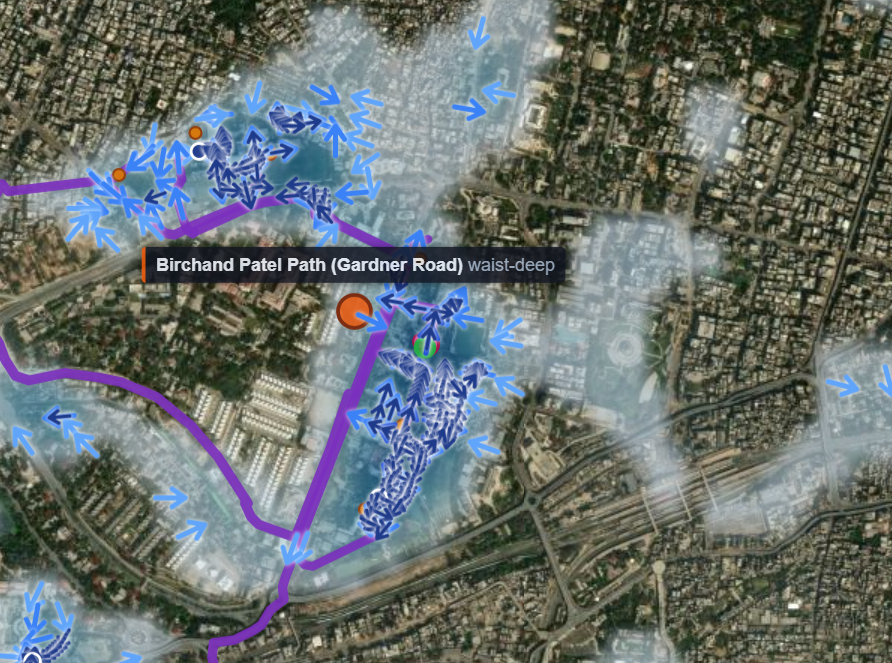
\includegraphics[width=0.99\linewidth]{figures/live_patna_route.png}
\caption{Flood-aware routing in the deployed system. The purple line is the recommended route,
orange circles are street nodes the router refuses to cross, the arrows are the predicted flow
field, and the label names the specific road that is impassable. The full-graph risk query behind
this view takes about 4\,ms, which is why the route updates as the rainfall slider moves.}
\label{fig:route}
\end{figure}

\subsection{Honesty and deployment}
FloodGNN distils the twin, so it inherits the twin's biases. Its claims are amortization, routing
quality \emph{under} the twin's flood fields, and transfer. They are not co-location skill, which
Section~\ref{sec:twin} shows the twin itself largely lacks and which a model learned directly from
terrain does have. Supervising directly on radar-observed street water is the natural next step and
we have not done it.

The 1.8\,MB checkpoint ships inside the dashboard image. The routing endpoint answers from the GNN
where a checkpoint exists and from the raster emulator otherwise, and it reports which backend
answered.
